%! Author = mkeim
%! Date = 7/18/24

\section{RP1: Statistically Significant Detection of Linguistic Change} \label{sec:paper_kulkarni}
\subsection{Introduction} \label{subsec:kulkarni_introduction}

Kulkarni et al.\ (2015) explores the problem of detecting changes in word usage patterns over time.
They introduce methods to identify words that have undergone significant shifts in \emph{meaning}, usage \emph{frequency}, and \emph{context}.
This is achieved by analyzing historical corpora, which contain vast amounts of text data spanning multiple centuries.
The study utilizes diverse datasets, including Twitter posts, Amazon product reviews, and Google Book Ngrams, to construct time series for individual words.

The research conducted by Kulkarni et al.\ exhibits a compelling alignment with our own research objectives,
specifically focusing on the identification of \emph{data voids} characterized by shifting semantic meanings over time.
Their exploration into these linguistic shifts has revealed interesting insights, such as the evolution of the word `gay,' (\Cref{fig:kulkarni-example})
which transitioned from being cheerful or dapper to signifying homosexual or lesbian aspect around the mid-20th century.

\begin{figure}[htb]
    \centering
    \vspace{-1em}
    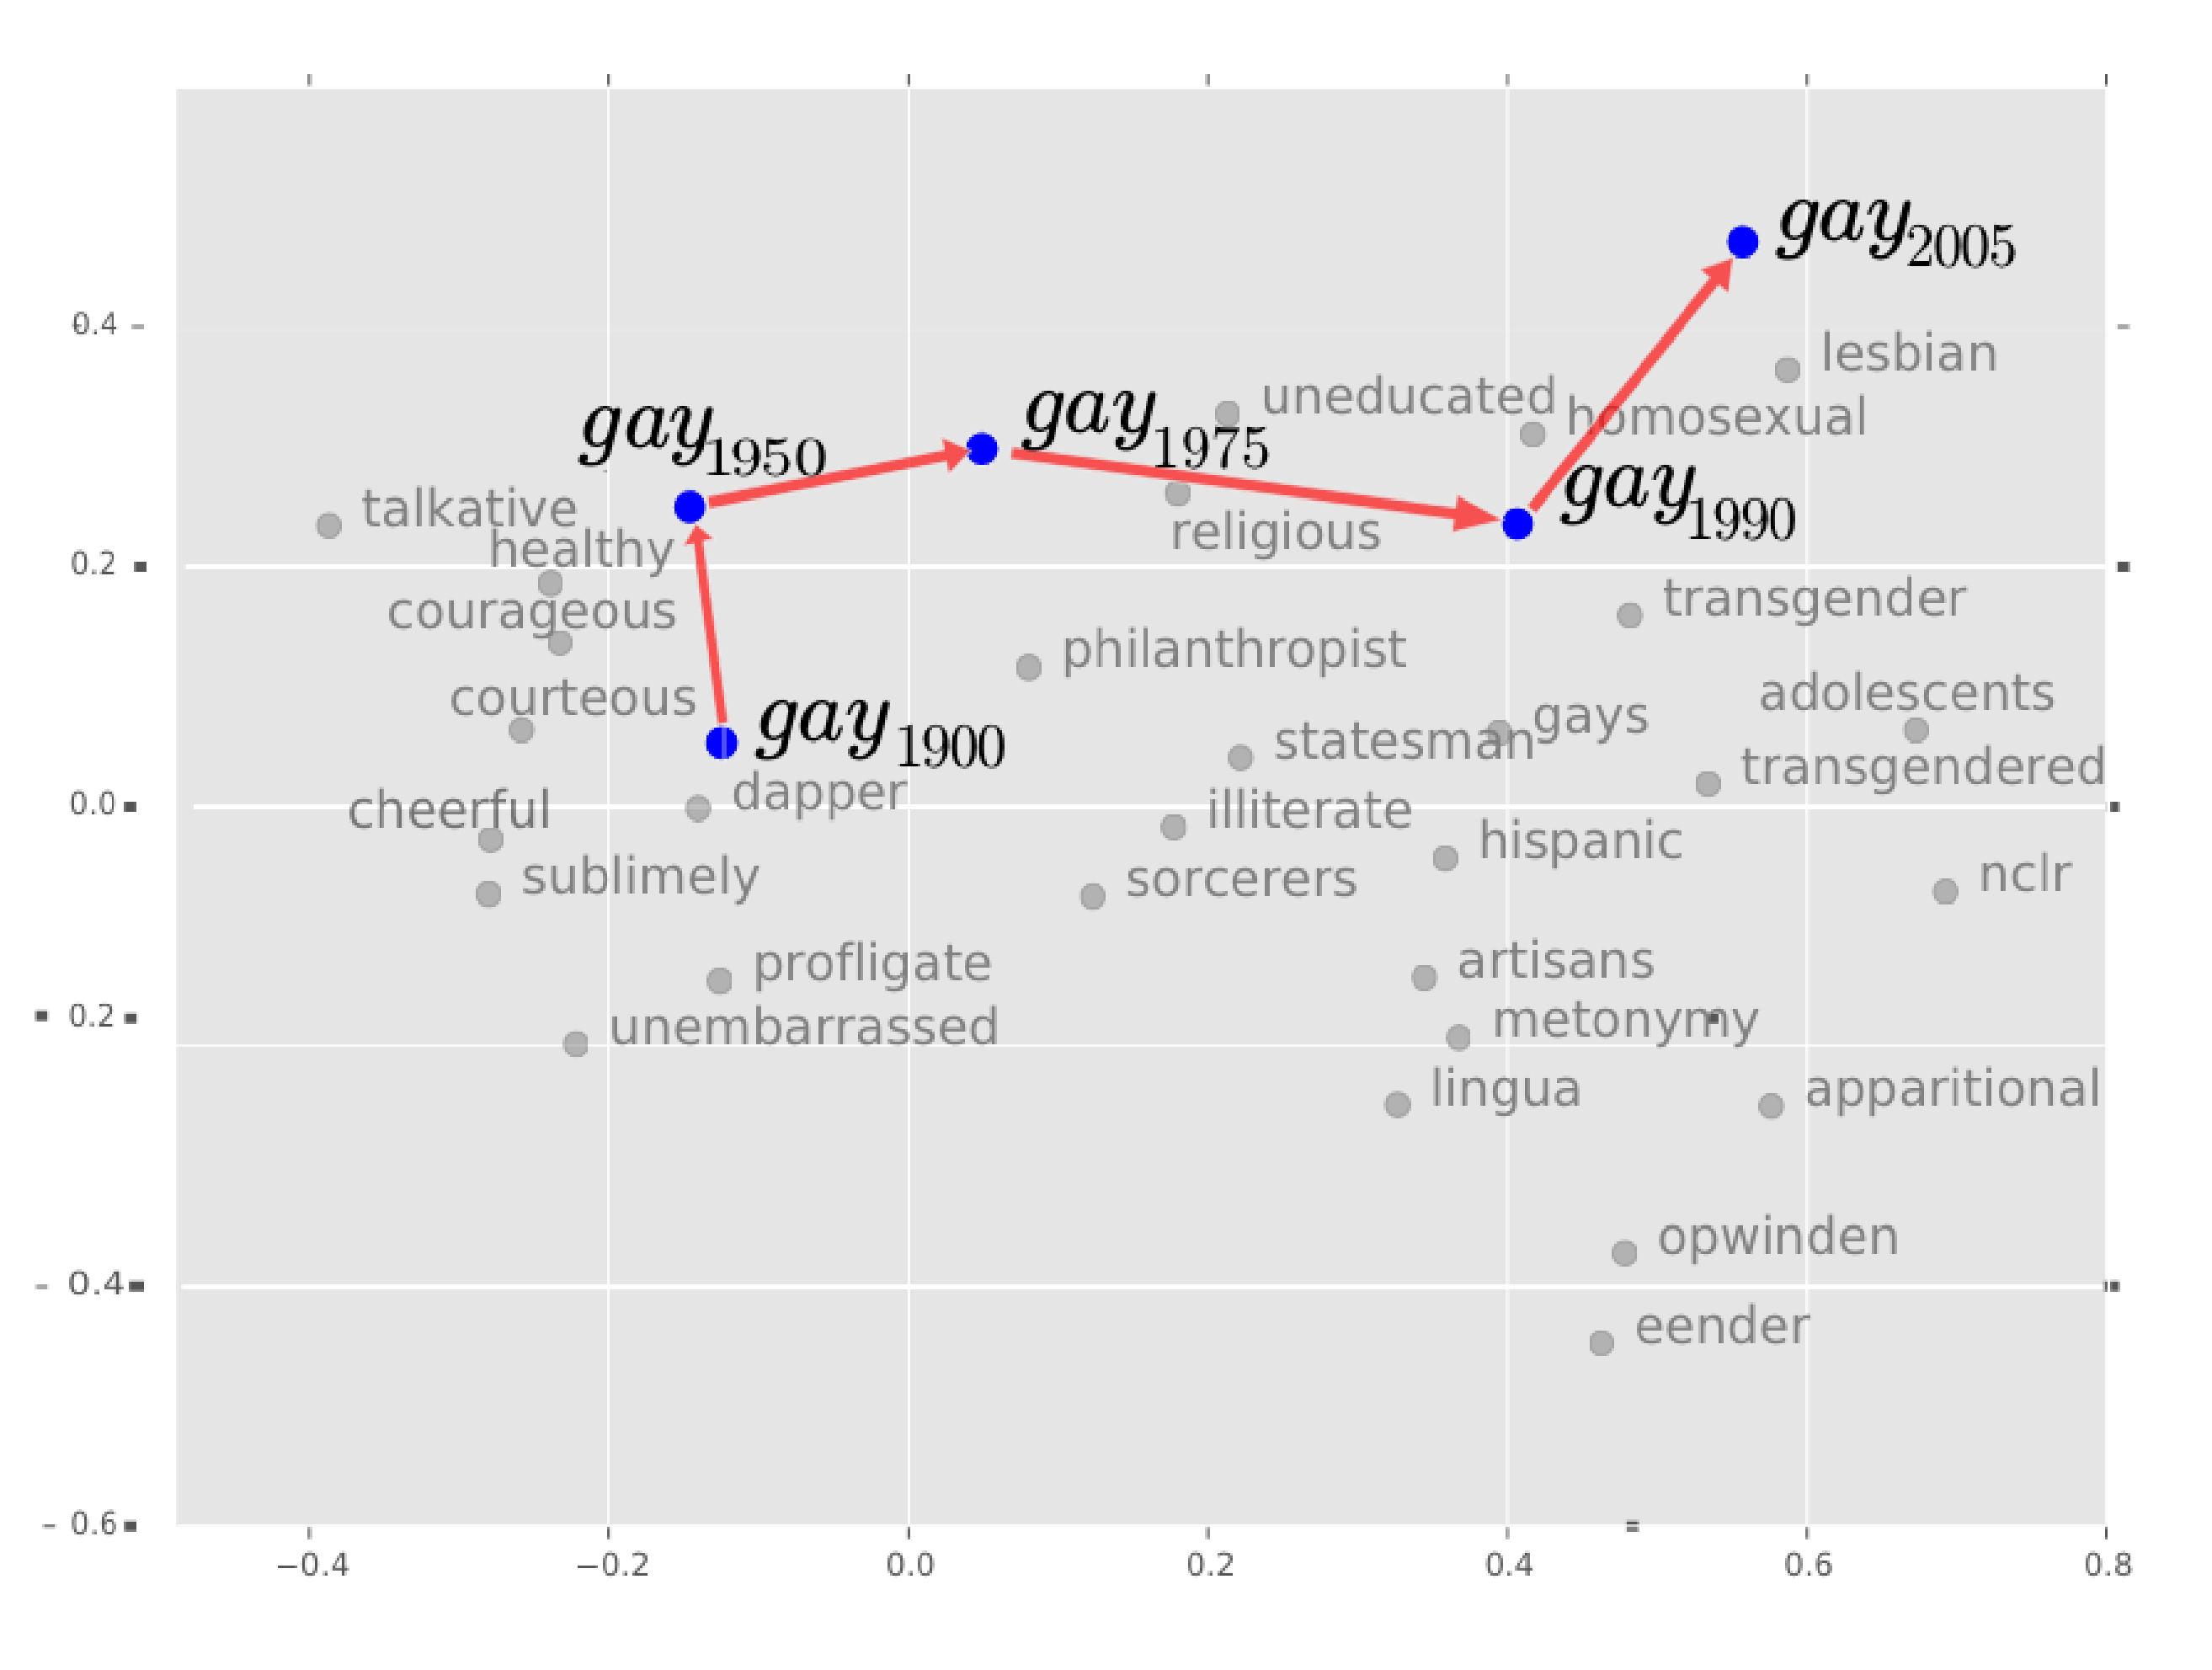
\includegraphics[scale=0.17]{figures/example-gay}
    \vspace*{-0.5cm}
    \caption{Example of word 'gay' undergoing change in meaning over time (taken from \cite{kulkarni2014statisticallysignificantdetectionlinguistic}).}
    \label{fig:kulkarni-example}
\end{figure}

To achieve understanding of this phenomenon, they studied the following research questions.
\begin{itemize}
    \item \para{RQ1.} \emph{What methods can quantify the statistical relevance of observed changes in a word's usage across different time periods?}\\
    Kulkarni et al.’s study uses three technical methods to understand how words change over time: \emph{frequency} analysis, \emph{syntactic} analysis, and \emph{distributional} analysis.
    The frequency method tracks how often words are used, revealing spikes in usage when significant events occur, like how \emph{breaking news} data voids can create a surge in specific keywords.
    The syntactic method looks at changes in the grammatical roles of words, while the distributional method examines word co-occurrence patterns to see how word meanings shift.
    Their approach not only uncovers the dynamic nature of language but also highlights “data voids,” -- areas where terms have \emph{evolved}, become \emph{outdated}, or \emph{fragmented} in meaning.

    \item \para{RQ2.} \emph{Given that a word's usage has changed, how can the precise moment or period of this shift be determined?}\\
    Understanding data voids involves not only recognizing that a change is occurring but also analyzing the specifics of how that change unfolds over time.
    It’s crucial to pinpoint not just the fact that a shift has happened, but also the exact moment when it took place.
    Kulkarni et al.\ tackle this challenge by implementing a \emph{change point detection algorithm} based on the \emph{Mean Shift} model.
    This method determines whether a word has experienced a significant shift and, if so, identifies the precise point at which this change occurred.
\end{itemize}

Next two sections, \Cref{subsec:kulkarni-rq1} and \Cref{subsec:kulkarni-rq2} focuses on the two research questions that this paper is studying, the approach they took to study and their results.

\subsection{What methods can quantify the statistical relevance of observed changes in a word's usage across different time periods?} \label{subsec:kulkarni-rq1}

\para{Overview.}
The challenge is to identify how the meaning of words changes over time.
To address this, they examine a corpus containing data from various domains like books, tweets, and reviews, known as the Temporal Corpus $(C)$ which spans over a time period $(S)$.
This corpus is divided into smaller segments called snapshots $C_t$, each of length $P$.
From these snapshots, a common vocabulary $V$ is created having words which are common across all snapshots.
To analyze changes in these words, a time series $T(w)$ is constructed for each word $w\in V$ (\Cref{fig:kulkarni-overview}).

Kulkarni et al.\ propose several methods to create this time series, aimed at understanding the evolution of words over time.

\begin{figure}[!h]
    \centering
    \vspace{-1em}
    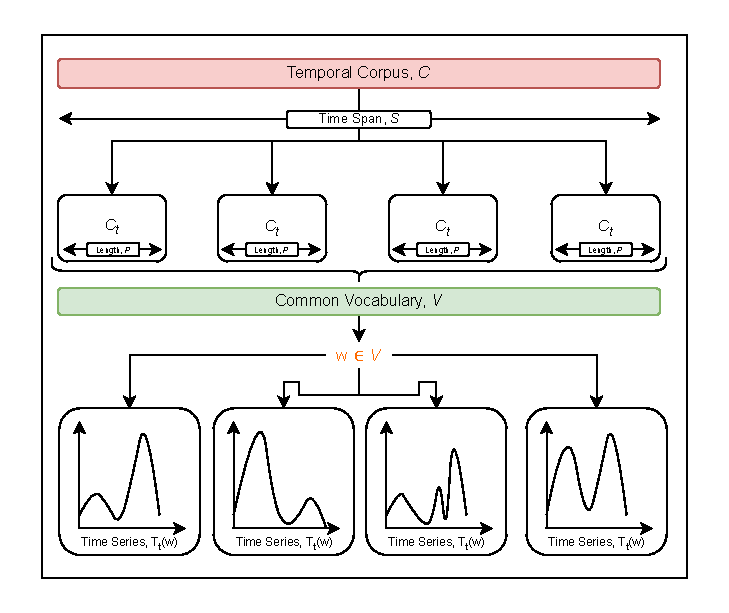
\includegraphics[scale=0.8]{figures/kulkarni_drawio}
    \vspace*{-0.7cm}
    \caption{Overview of time series construction.}
    \label{fig:kulkarni-overview}
\end{figure}

\para{Construction of time series.}
In this paper, three methods are explored for statistically modeling the evolution of words over time:
frequency analysis, part-of-speech tagging, and word co-occurrence to create time series for each word.

\begin{wrapfigure}{r}{0.3\textwidth}
    \centering
    \vspace{-3em}
    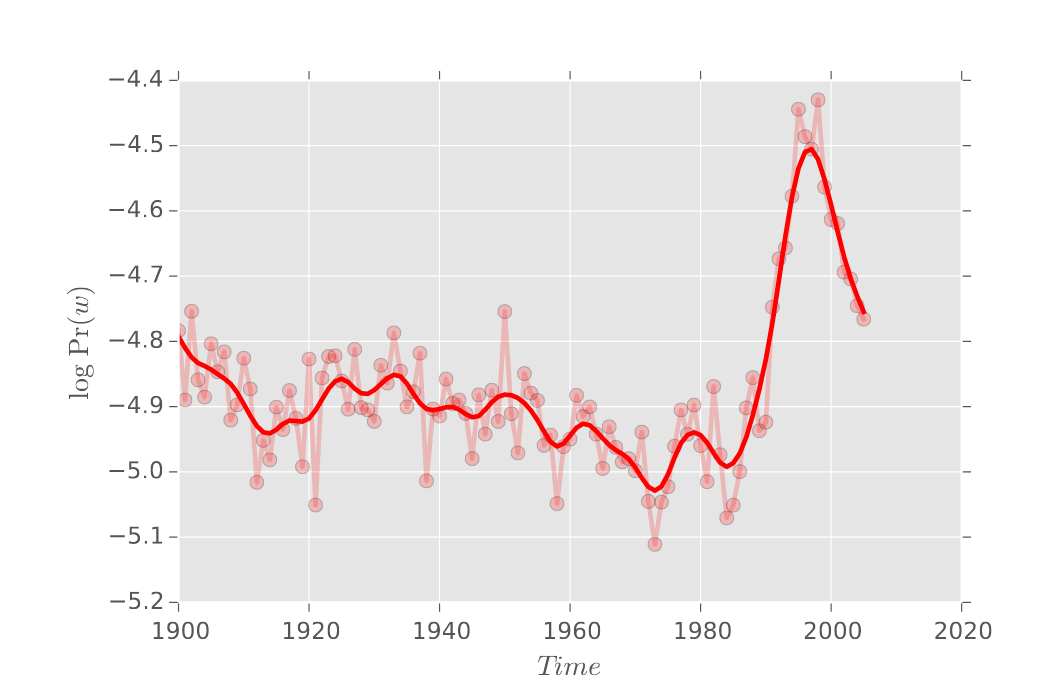
\includegraphics[width=0.35\textwidth]{figures/frequency-gay}
    \vspace*{-1cm}
    \caption{Changes in frequency of 'gay' (taken from \cite{kulkarni2014statisticallysignificantdetectionlinguistic}).}
    \label{fig:example-gay}
\end{wrapfigure}

\para{Frequency method.}
The simplest and most direct method for detecting sudden changes in word usage is by analyzing frequency trends.
This approach examines how often a word is used over a given period, providing insights into shifts in its popularity or relevance.
Changes in frequency can indicate whether a word is gaining new meanings or losing old ones, reflecting broader cultural or societal trends.
For example, the word “gay” in \Cref{fig:example-gay} shows a noticeable spike in usage during the 1980s, signaling a shift in its meaning or cultural relevance.

Tools such as the Google Books Ngram Viewer and Google Trends are used for this purpose, as they provide large datasets and visual representations of word usage across different timeframes.
They calculate the change in probability of a word appearing over time.
\begin{equation}
\mathbf{T_t(w)} = \log \frac{#(w \in C_t)}{|C_t|}
\label{eq:equation}
\end{equation}

\para{Syntactic method.}
Frequency-based metrics, while simple to compute, are susceptible to errors caused by imbalances in the corpus's domain and genre distribution.
Fluctuations in word usage due to temporal events or the popularity of specific entities can obscure genuine shifts in word meaning.
Moreover, a word's grammatical role can evolve over time, such as acquiring a different part of speech category.
To study this, the corpus is annotated with part-of-speech (POS) tags, and the probability distribution of these tags is calculated for each word across different time snapshots.
This approach allows researchers to observe how a word’s syntactic role changes over time.

\para{Distributional method.}
For detecting subtle semantic changes, which are not changed either due to frequency or through change in part of speech,
this method was developed to understand in which context a word is used in and based on that understand the semantic changes.
Distributional methods focusses on creating a semantic space that maps words to continuos vector space, where each word is represented by a vector.
Once they created a temporal word embeddings for each word in each time snapshot, then they track the changes of the represtantations across the embedding space.

The researchers aimed to \emph{learn word embeddings} by training neural language models on a corpus at different time snapshots.
They initialized word vector representations randomly and optimized the model parameters using stochastic gradient descent.
During training, the objective was to maximize the probability of context words appearing around a target word.
After training, word embeddings were normalized by their L2 norm to ensure consistent representation.

The \emph{alignment} process involved aligning word embeddings from different time snapshots into a unified coordinate system to characterize changes between them.
Assumptions were made to aid the alignment process, including the equivalence of spaces under linear transformation and the preservation of local structure of most words over time.
When the alignment model failed to align a word correctly, it indicated a potential linguistic shift, highlighting the importance of accurate alignment for tracking semantic changes over time.
By aligning embedding spaces across various time snapshots into a joint embedding space,
the distributional method constructs a \emph{distributional time series} that captures the semantic evolution of words over time.

The paper shows the evolution of the word `tape' over time.
Initially, the word `tape' referred to an `adhesive tape' but underwent a semantic shift to also mean a `cassette tape'.

\subsection{Takeaways}\label{subsec:takeaways}
For the first research question, Kulkarni et al.\ (2015) explored multiple dimensions of word usage change over time.
To address this, they constructed three types of time series: frequency-based, syntactic, and distributional.

Frequency-based method relies on analyzing the frequency of word usage over time.
It provides immediate insights into trends and spikes in word usage.
However, the frequency method is prone to sampling errors, it may indicate a change in frequency without a significant shift in meaning,
as seen with the word `Hurricane' during events like Hurricane Sandy, where frequency increased but meaning remained stable.
Syntactic-based method analyzes the part of speech (POS) tags of words to detect changes in their syntactic roles over time.
Distributional-based method is based on the fact that words appearing in similar contexts are semantically similar.

Among the three methods employed by Kulkarni et al.\ (2015) for constructing time series,
the distributional time series proved most insightful, as it captures the contextual usage of word.
This approach utilized word embeddings to capture the semantic context of a word within specific time periods.

The syntactic method, while reliable in detecting changes in part-of-speech tags, may overlook significant shifts due to its reliance on linguistic taggers.
At the time of the study, this posed a challenge due to the limitations of tagging accuracy, which has since improved significantly with the advent of more advanced methods for annotating datasets with POS tags.

%back-propogation alogithm
%normalization factor
%negative lof-likelihhod
%stochastic gradient descent
%L2 Norm

\subsection{Given that a word's usage has changed, how can the precise moment or period of this shift be determined?} \label{subsec:kulkarni-rq2}
The authors introduce a method for identifying significant changes in word usage over time using a \emph{change point detection algorithm} based on the \emph{Mean Shift model}.
The process begins by constructing time series data for each word in the corpus—whether using frequency-based, syntactic, or distributional methods.
The next step is to determine if the word has experienced a significant change.
If a significant shift is detected, the algorithm then identifies and returns the \emph{estimated change point (ECP)}, which marks the time when this change occurred.

Since language exhibits a stochastic drift.
In this context, `stochastic' refers to the randomness or probabilistic nature of the training process,
where the models are trained on the same dataset but may produce different results each time due to this randomness.
To resolve this, time series was normalized for each word by transforming the time series into a \emph{Z-score series}.

The Mean Shift model is then applied, which involves calculating the mean of the time series data before and after each potential change point.
By comparing these means, the algorithm determines if a statistically significant change has occurred at any given point in time.

%\begin{figure}[htb]
%    \centering
%    \vspace{-1em}
%    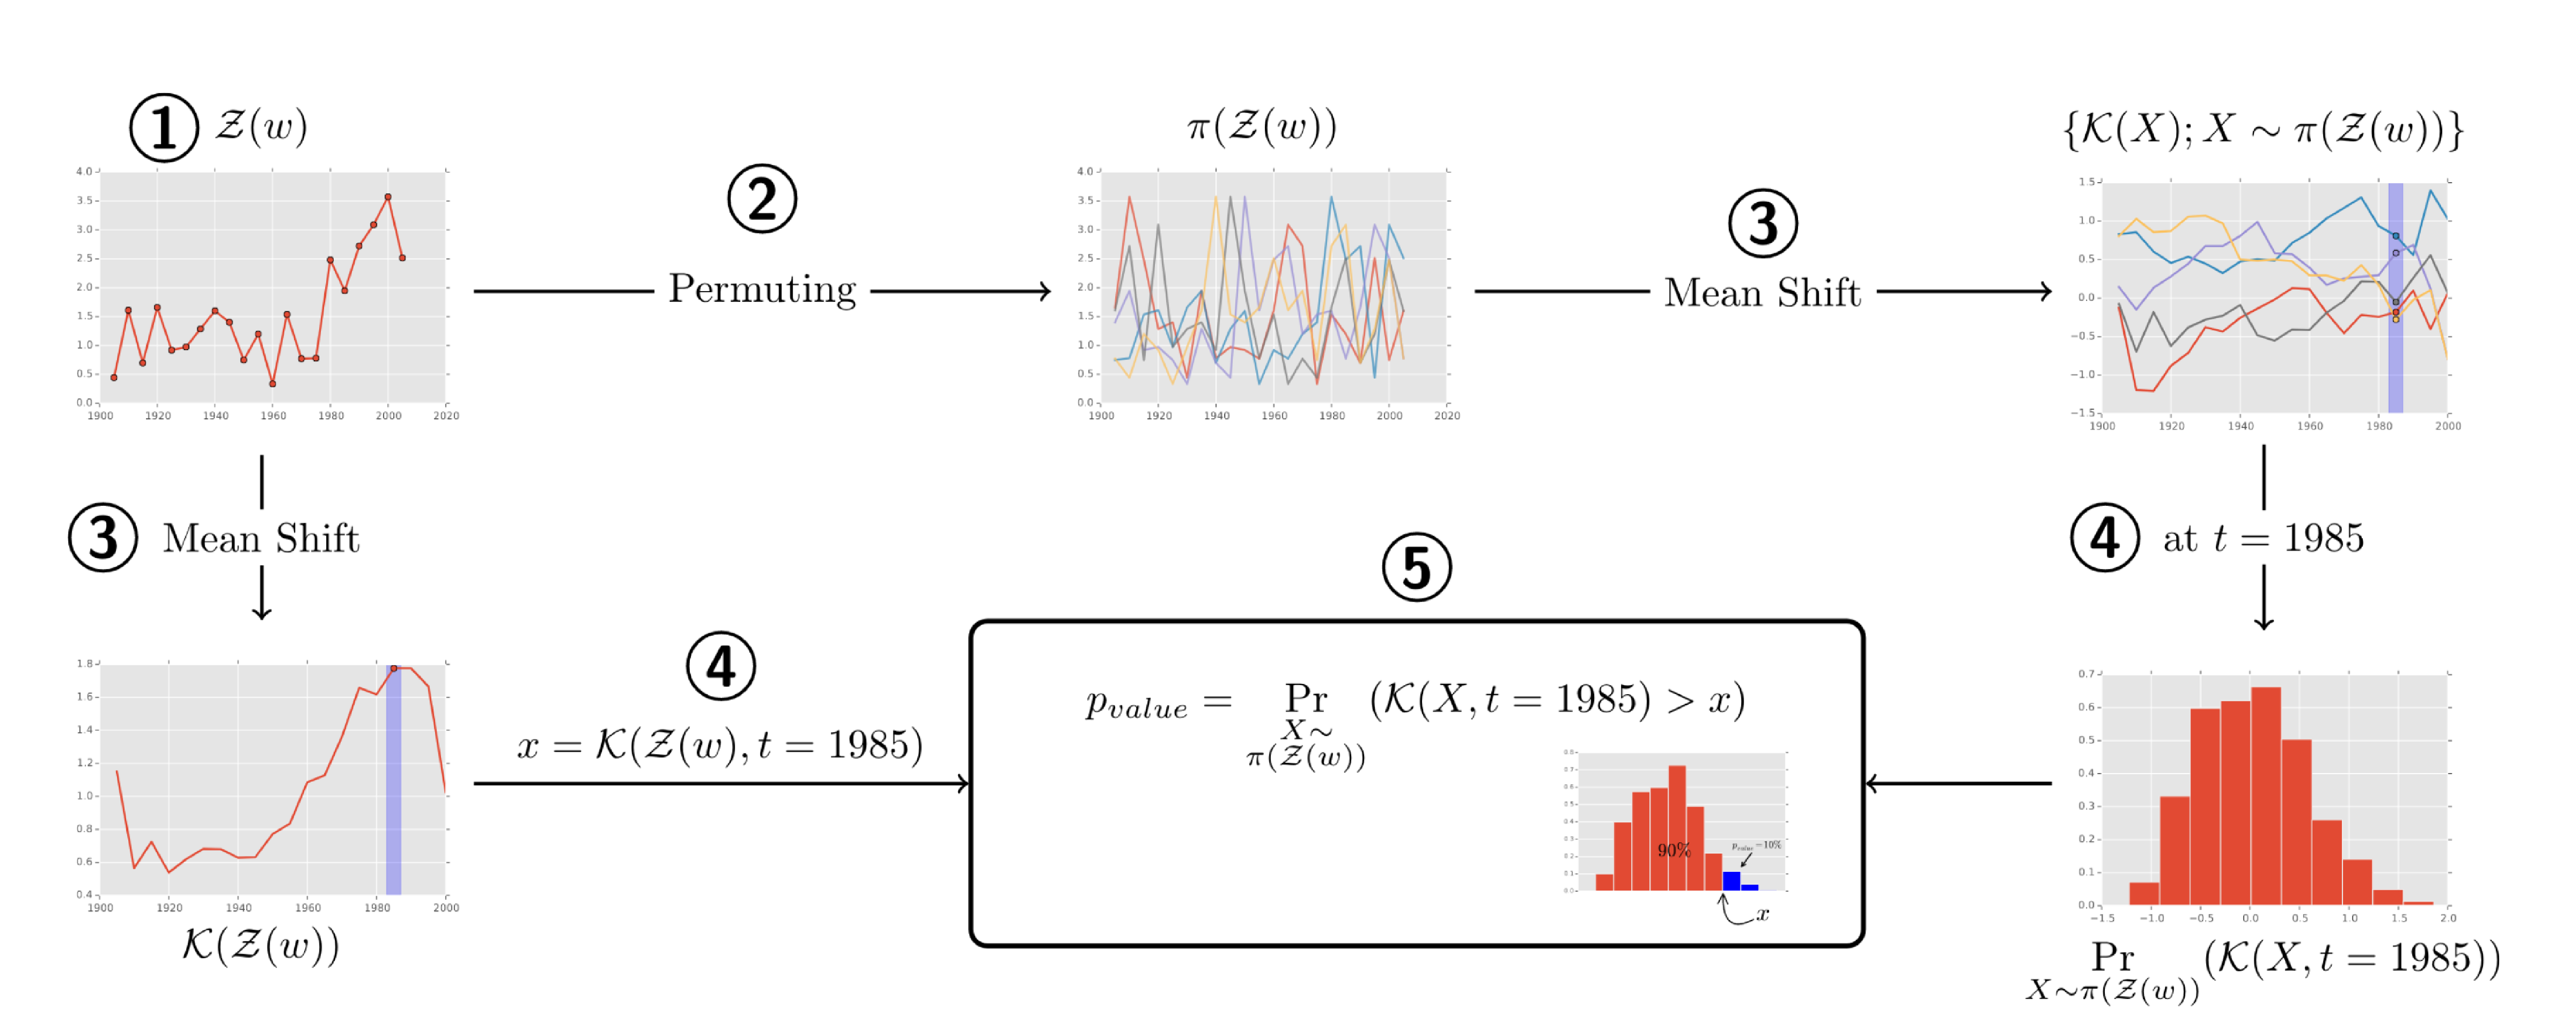
\includegraphics[scale=0.17]{figures/changepoint}
%    \vspace*{-0.5cm}
%    \caption{Change Point Algorithm (taken from \cite{kulkarni2014statisticallysignificantdetectionlinguistic}).}
%    \label{fig:kulkarni-changepoint}
%\end{figure}

\para{Change point algorithm.}
After constructing time series data for each word in the corpus—whether using frequency-based, syntactic, or distributional methods (\Cref{subsec:constructing-word-embeddings}), the first step is to normalize the time series data for the word $w$.
After normalization, the algorithm computes a mean shift series, denoted as $K(Z(w))$.
The \emph{mean shift} is defined as the difference in the mean of a time series at different time points.
The algorithm calculates this shift by segmenting the time series around a pivot point, denoted as time point $j$, and comparing the means of the segments before and after this point.
To assess the significance of the computed mean shifts, the algorithm employs a \emph{bootstrapping} method.
The algorithm uses bootstrap samplingto estimate how likely an observed shift is, under the assumption that no real change has occurred (the null hypothesis).
It generates multiple time series by randomly resampling the original time series, denoted as $BS$.
This is done by repeatedly drawing samples from the normalized data $Z(w)$ until the number of samples equals $B$, which is predefined.
The p-value is then calculated by comparing the observed mean shift to the distribution of mean shifts from the bootstrapped samples.
It reflects the proportion of times that the mean shift from the random (permuted) samples exceeds the observed mean shift.
A low p-value indicates that the observed shift is unlikely to be due to random fluctuations alone.
The algorithm identifies potential change points by looking for times $j$ where the Z-Score $Z_j(w)$ is greater than or equal to the threshold $\gamma$,
which is set to the 96th percentile, to filter out less significant potential change points.
It then checks the p-values for these change points and selects the one with the smallest p-value, indicating the most significant change.
The algorithm returns the p-value and the estimated change point (ECP).
This information helps understand exactly when the meaning or usage of the word has shifted over time.
%\Cref{fig:kulkarni-changepoint} illustrates the important aspects of the algorithm.

\subsection{Takeaways}\label{subsec:takeaways2}
The change point detection algorithm (\Cref{subsec:kulkarni-rq2}) presented in the paper detects significant linguistic shifts over time by analyzing word time series data.
To detect changes, they first convert these time series into Z-score series, which normalize the data and make it easier to identify shifts.
The Mean Shift model is then applied, which involves calculating the mean of the time series data before and after each potential change point.
By comparing these means, the algorithm determines if a statistically significant change has occurred at any given point in time.

The paper illustrates this with the example of the word `tape,' which transitioned from meaning adhesive tape to cassette tape, with the change detected in the \emph{1970s}.
Similarly, the word `apple' shifted from being used primarily as a common noun to a proper noun associated with Apple Inc., with this change occurring around \emph{1984}.

These examples illustrate the algorithm’s capability to pinpoint when a word’s usage and meaning undergo significant shifts.
The paper emphasizes the importance of analyzing these changes to understand linguistic evolution better.

\subsection{Results} \label{subsec:kulkarni-results}

\para{Time series analysis \& historical analysis.}
The results presented in Kulkarni et al.\ (2015) illustrate how words acquire new meanings and how these meanings change over time through time series and historical analysis.

\para{Frequency method.}
For words like `transmitted,' `bitch,' `sex,' and `her,' the frequency and distributional methods reveal significant insights.
For example, the sharp increase in the frequency of the word `her' around the 1960s can be attributed to the concurrent rise of the feminist movement.
However, the frequency method can produce many false positives due to the temporary popularity of specific social and political events.

\begin{table}[tbh]
\begin{tabular}{@{}lllll@{}}
\toprule
\textbf{Method}         & \textbf{Examples}                              &  &  &  \\ \midrule
\textbf{Frequency}      & transmistted, bitch, sex, her                  &  &  &  \\
\textbf{Syntactic}      & apple, hug, sink, click, handle, windows, bush &  &  &  \\
\textbf{Distributional} & diet, tape, plastic                            &  &  &  \\ \bottomrule
\end{tabular}
\caption{Time Series Analysis}
\label{tab:time-series-examples}
\end{table}
\raggedbottom

\para{Syntactic method.}
The syntactic method uniquely detected the word `apple,' which saw its most frequent part of speech tag shift significantly from `Noun' to `Proper Noun.'
This method has a low false positive rate but suffers from a high false negative rate, as evidenced by its detection of only two words in the study.

\para{Distributional method.}
For words like `diet,' `tape,' and `plastic,' the distributional method sheds light on significant changes in their usage.
The popularity of dieting books, starting with the bestseller `Dr. Atkins’ Diet Revolution' by Robert C. Atkins in 1972, shifted the meaning of `diet' from simply referring to the food consumed to a lifestyle of food consumption behavior.

These findings demonstrate the nuanced ways in which word meanings evolve and the strengths and limitations of different methods in detecting these changes.
\Cref{tab:time-series-examples} shows all the examples that the paper have shown for different methods.
While frequency and distributional methods can highlight shifts in usage, they are prone to false positives.
The syntactic method, though precise, may miss many significant changes.
Therefore, a combined approach utilizing all methods may offer the most comprehensive insights into linguistic evolution

\para{Cross domain analysis.}
The study extends its analysis to datasets like Amazon Reviews and Twitter, which cover much shorter time scales compared to the Google Books Ngram Corpus.
This cross-domain analysis explores the impact of applying the distributional method on these more temporally constrained datasets.
\Cref{tab:sources-examples} presents words that exhibit semantic change across various datasets.

\begin{table}[tbh]
\begin{tabular}{@{}lllll@{}}
\toprule
\textbf{Dataset Source} & \textbf{Examples}                     &  &  &  \\ \midrule
\textbf{Amazon Reviews} & streaming, ray, combo, rays, twilight &  &  &  \\
\textbf{Twitter Tweets} & candy, myster, rally, sandy           &  &  &  \\ \bottomrule
\end{tabular}
\caption{Cross Domain Analysis}
\label{tab:sources-examples}
\end{table}
\raggedbottom

In the Twitter dataset, the word `sandy' acquired a new sense following Hurricane Sandy hitting the East Coast of the USA\@.
Similarly, the analysis on Amazon Reviews revealed changes in words associated with new products and technology trends.

These words demonstrate the method’s ability to capture emerging usages and meanings.
The example of `sandy' highlights how a natural disaster can influence linguistic shifts, with the word gaining a new context and meaning after the hurricane event.

These examples demonstrate that the method can effectively detect the introduction of new products, movies, and books, showcasing its adaptability to different domains and time scales.
This cross-domain capability is particularly valuable for identifying and understanding contemporary linguistic changes in rapidly evolving contexts like social media and online reviews.

\subsection{Takeaways} \label{subsec:kulkarni-takeaways}
The paper by Kulkarni et al.\ (2015) presents an innovative approach to detecting significant linguistic changes over time using statistical methods and word embeddings.
The goal behind their work is to systematically track and analyze how words evolve in meaning and usage across different temporal contexts.
They construct time series for each word using three distinct methods:
frequency, which captures the prevalence of word usage over time;
syntactic, which examines shifts in part-of-speech tags;
and distributional, which looks at changes in word co-occurrence patterns.
They also employ a change point detection algorithm which identifies estimated change points, where significant linguistic shifts occur.
Their analysis spans various datasets, including Google Books Ngram Viewer, Amazon Reviews, and Twitter,
demonstrating the method’s adaptability and effectiveness in detecting both gradual and abrupt changes in word meanings across different domains and time scales.